\documentclass[preview,biblatex]{ctsDIGI}

\usepackage[spanish,es-nodecimaldot,es-tabla]{babel}
\usepackage[utf8]{inputenc}
\usepackage{csquotes}
\DeclareLanguageMapping{spanish}{spanish-apa}
\addbibresource{bibliografia.bib}

\usepackage{lipsum}

%----------------------------------------------------------------------------------------
%	TITLE SECTION
%----------------------------------------------------------------------------------------

\titleSp{Título en español}
\titleEn{English title}
\shorttitle{Título corto}


\author{A.Fulano*, B. Mengano}
\affiliation{Escuela de ciencias Físicas y Matemáticas, Universidad de San Carlos de Guatemala, Guatemala}
\contactmail{aful@ecfm.usac.edu.gt}
%----------------------------------------------------------------------------------------
%	ABSTRACTS & KEYWORDS
%----------------------------------------------------------------------------------------

\abstractSp{\bl{A} loren \lipsum[1]}
\keywordsSp{Primera, Segunda, Tercera, Cuarta, Quinta}

\abstractEn{\bl{E} loren \lipsum[1]}
\keywordsEn{Frist, Second, Third, Fourth, Fifth}

%----------------------------------------------------------------------------------------

\begin{document}

\maketitle


%----------------------------------------------------------------------------------------
%	ARTICLE CONTENTS
%----------------------------------------------------------------------------------------



\section{Introducción}
En este párrafo se muestra como son la referecias a tablas (Ver Tabla \ref{table:resumen}), figuras (Ver Figura \ref{fig:Arreglo}) y bibliografía (\cite{Maldacena:2016upp}).

\lipsum[1]

\section{Materiales y métodos}
\lipsum*[1](\cite{Aparicio:2016qqb})

\subsection{Subsección}
\lipsum*[1]
\begin{equation}
a^2 = b^2 + c^2 -2bc\cos\theta
\end{equation}
\lipsum[1]

\section{Resultados}
\lipsum*[1](\cite{halliday1986fundamentos})

\begin{table}
\begin{center}
\caption{Esta es la descripción (\emph{Caption}) de la tabla} \label{table:resumen}
\begin{threeparttable}
{\sizeNueveymedio
\begin{tabular}{c c c}
\hlinec
Columna 1 & Columna 2 & Columna 3 \tnote{$^\diamond$} \\
\hlinec
Fila 1	& $m$&	1\\
Fila 1	&$q$&	2 \tnote{$^\ddag$} \\
Fila 1	&$s$&	3\\
Fila 1	&$\tau$ & 4\\
\hlinec
\end{tabular}}
\smallskip
{\scriptsize
\begin{tablenotes}
\item \textit{Nota} $\diamond$: Primera nota de la tabla.
\item \textit{Nota} $\ddag$: Segunda nota de la tabla.
\end{tablenotes}
}
\end{threeparttable}
\end{center}
\end{table}

\lipsum*[1]

\section{Discusión}
\lipsum*[1](\cite{knoll2010radiation})

\begin{figure}
\centering
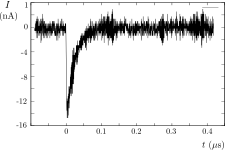
\includegraphics{figura.pdf}
\caption{Esta es la Descripción de la figura.}
\label{fig:Arreglo}
\end{figure}

\lipsum[1]


\section{Agradecimientos}
\lipsum[1]

\ctsDIGIprintbibliography

\par\leavevmode
\end{document}
